\pagenumbering{arabic} %necessary to start numbering pages in arabic numerals from here
\setcounter{page}{1} 


{\Huge \bfseries \noindent Chapter 1}
\vspace{-1em} 
\section*{\LARGE Introduction}
\addcontentsline{toc}{section}{1\quad Introduction}
\setcounter{section}{1} % ensure next subsection starts at 1
\renewcommand{\chapternum}{1}

% Reset figure/table numbering per chapter
\renewcommand{\thefigure}{\chapternum.\arabic{figure}}
\setcounter{figure}{0}
\renewcommand{\thetable}{\chapternum.\arabic{table}}
\setcounter{table}{0}

\vspace{2em}

\subsection{Prostate structure and function}
The prostate is the major reproductive gland involved in male fertility. In pubescent males, the prostate gland is located in the pelvis below the urinary bladder, immediately anterior to the rectum. It plays a role in developing secondary male characteristics and subsequently supplements the seminal vesicles in producing seminal fluid for fertilisation \cite{Verze2016Jul}. Structurally, the prostate gland is approximately 3cm in length and 20g in weight in male adults \cite{Almeeri2024Nov}, divided into three zones: the central zone, the transition zone and the peripheral zone (Figure \ref{prostateanatomy}a). The transition zone represents the smallest component, accounting for 5-10\% of the glandular tissue, separated from the remaining components by a fibromuscular band of tissue. The central zone expands in a cone shape around the ejaculatory ducts, constituting 20-25\% of the gland. Finally, the peripheral zone represents the largest component (70\%), spanning the posterior and lateral components of the gland \cite{Verze2016Jul}. The fibromuscular tissue contracts to close the seminal ducts during urination, preventing backflow of bodily fluids, whilst during ejaculation, the fibrous muscles work in concert with the sphincter muscle to prevent semen from entering the bladder \cite{IQWiG2022Sep}. On a microscopic level, the prostate gland contains stromal and epithelial compartments (Figure \ref{prostateanatomy}b). The epithelial layer is composed of luminal and basal epithelial cells, the former responsible for secreting prostate-specific antigen (PSA), and is interspersed with neuroendocrine cells. The stromal layer contains fibroblasts, myofibroblasts and smooth muscle cells, separated from the epithelial layer via an extracellular matrix termed the basement membrane \cite{Pitzen2023Apr}. Signalling between the epithelial and stromal cells maintains normal prostate development, homeostasis and regeneration, mediated via the androgen receptor (AR), bone morphogenic proteins (BMPs), wingless-type integration site (WNT), transforming growth factor $\beta$ (TGF-$\beta$), amongst others \cite{Prins2008May}. PSA production via the epithelium in prostatic tissue reduces seminal viscosity by degrading semenogelin and fibronectin, enhancing sperm migration to the cervix, and promoting overall fertility \cite{Lilja1988}. \iffalse Increased PSA levels occur naturally with age, however, increased PSA levels are also a marker of prostate cancer (PCa). PCa cells produce less PSA than benign cells; malignant PCa cells lack the basal layer that otherwise restricts the extravasion of PSA to the prostatic ducts and bloodstream \cite{David2024Sep}. As both benign and malignant prostate conditions elevate PSA levels, its use as a screening tool has become controversial, leading to unnecessary biopsies and overdiagnosis. Despite this, PSA screening remains the most useful marker for evaluating the extent of malignancy, identifying biochemical recurrences and monitoring disease progression \cite{David2024Sep}. \fi

\begin{figure}
    \begin{center}
        %\includegraphics[angle=90,origin=c,width=\textwidth, height=0.7\textheight,keepaspectratio]{Figure1.png}
        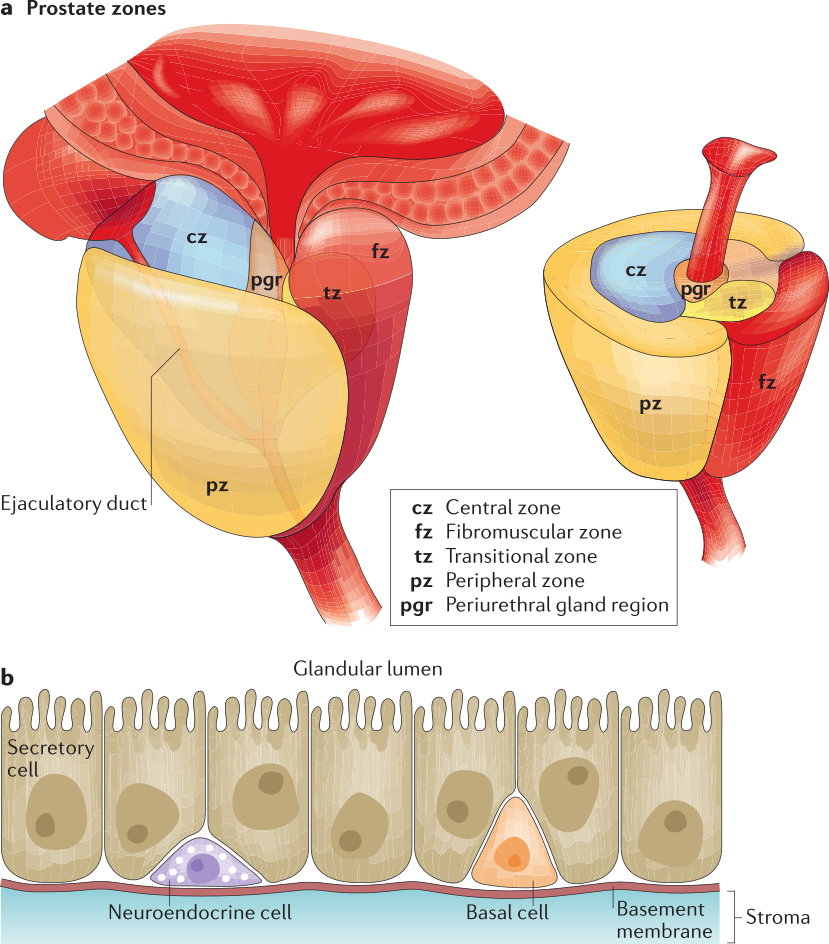
\includegraphics[keepaspectratio,width=\textwidth]{Introduction/Figures/prostateanatomy.png}
        \caption[Anatomy of the prostate gland]{\textbf{Anatomy of the prostate gland}. (\textbf{a}) General anatomical structure of the prostate. (\textbf{b}) Microscopic structure of the prostate. Permission granted for reuse from Springer Nature under license number 5982481051990 \cite{Verze2016Jul}}
        \label{prostateanatomy}
    \end{center}
\end{figure}

\subsubsection{Androgens and AR in prostate development and homeostasis}
The growth of the prostate begins in the foetus and is complete at sexual maturity. The prostate develops from the urogenital sinus (UGS), an epithelial-mesenchymal structure located at the base of the developing bladder, which, at 10-12 weeks postconception, commences prostatic morphogenesis via circulating androgens produced by the fetal testis \cite{Hamilton1959}. In females, the absence of androgens dictates that the UGS forms the lower portion of the vagina and the urethra. Initial prostatic morphogenesis occurs via the growth of epithelial buds from the urogenital sinus epithelium (UGE) into surrounding urogenital sinus mesenchyme (UGM), forming precise patterns of epithelial cords establishing lobular subdivisions of the prostate (Figure \ref{prostatedevelopment}) \cite{Timms1994May}. The epithelium then reorganises into two distinct cell populations: basal epithelial cells located along the basement membrane and tall, luminal cells (Figure \ref{prostateanatomy}b). During this time, the prostatic stroma differentiates into smooth muscle layers surrounding the prostatic ducts \cite{Wang2001Oct}. Once fully formed, the prostate does not undergo exponential differentiation again until puberty, when it reaches its mature size, shifting from stromal AR expression to epithelial AR expression (Figure \ref{prostatedevelopment}). Despite sustained levels of circulating androgens post-puberty, AR signalling in both the epithelium and stroma transitions from growth to a steady-state phase \cite{Vickman2020Jul}. Androgens, namely testosterone, are primarily secreted from the testis and, upon uptake by prostatic cells, are converted to dihydrotestosterone (DHT) via 5$\alpha$-reductase. DHT binds to the AR with two- to five-fold higher affinity than testosterone, yielding 10-fold AR signalling \cite{Gao2005Sep}. Therefore, androgen availability, AR expression and 5$\alpha$-reductase activity are all crucial to normal prostate development. In sexually mature males, the AR remains critical for the maintenance of the prostate. It has been demonstrated that following involution of the prostate, supplementation of androgens restores the prostate to its original size \cite{Isaacs2008Jun}.\par
The AR gene is located on the X chromosome and, like other members of the nuclear receptor family, the AR consists of three functional domains: the N-terminal domain (NTD), the DNA-binding domain (DBD) and the C-terminal ligand-binding domain (LBD), connected to the DBD via a hinge region \cite{Mangelsdorf1995Dec}. The highly conserved DBD links the AR to the promoter and enhancer regions of AR-mediated genes by direct DNA binding, allowing the NTD and LBD to activate transcription of AR genes, maintaining canonical differentiation. Defects in the AR gene can lead to dysregulation in the ratio between proliferation and cell death, of which androgen and AR are master regulators \cite{Denmeade1996Apr}. Defects of the AR gene can be caused by 1) point mutations causing substitutions or premature stop codons, 2) insertions and deletions (INDELs) causing frameshift mutations, 3) complete or partial gene deletion and 4) intronic mutations in splice sites affecting AR RNA splicing \cite{McPhaul2002Dec}. Progression towards prostate cancer (PCa) can be attributed to several AR-linked growth-promoting pathways. In $\sim$50\% of PCa tumours, gene fusions between \textit{TMPRSS2} and ETS family of transcription factors (ETS Transcription Factor ERG (\textit{ERG}) and ETS variant transcription factor 1) confer androgen responsiveness to members of the ETS family, resulting in cell-cycle progression \cite{Rubin2011Aug}. Three well-known cancer pathways (PI3K, Ras-Raf-MEK-ERK, RB) were shown to be dysregulated in primary PCa, however, analysis of AR pathway-associated genes revealed greater alterations when compared to other pathways, suggesting AR is indeed the master-regulator of PCa \cite{Taylor2010Jul}. The reliance of PCa on AR pathway perturbations is the rationale for the use of androgen deprivation therapy to treat PCa, as discussed in the following sections. 

\begin{figure}
    \begin{center}
        %\includegraphics[angle=90,origin=c,width=\textwidth, height=0.7\textheight,keepaspectratio]{Figure1.png}
        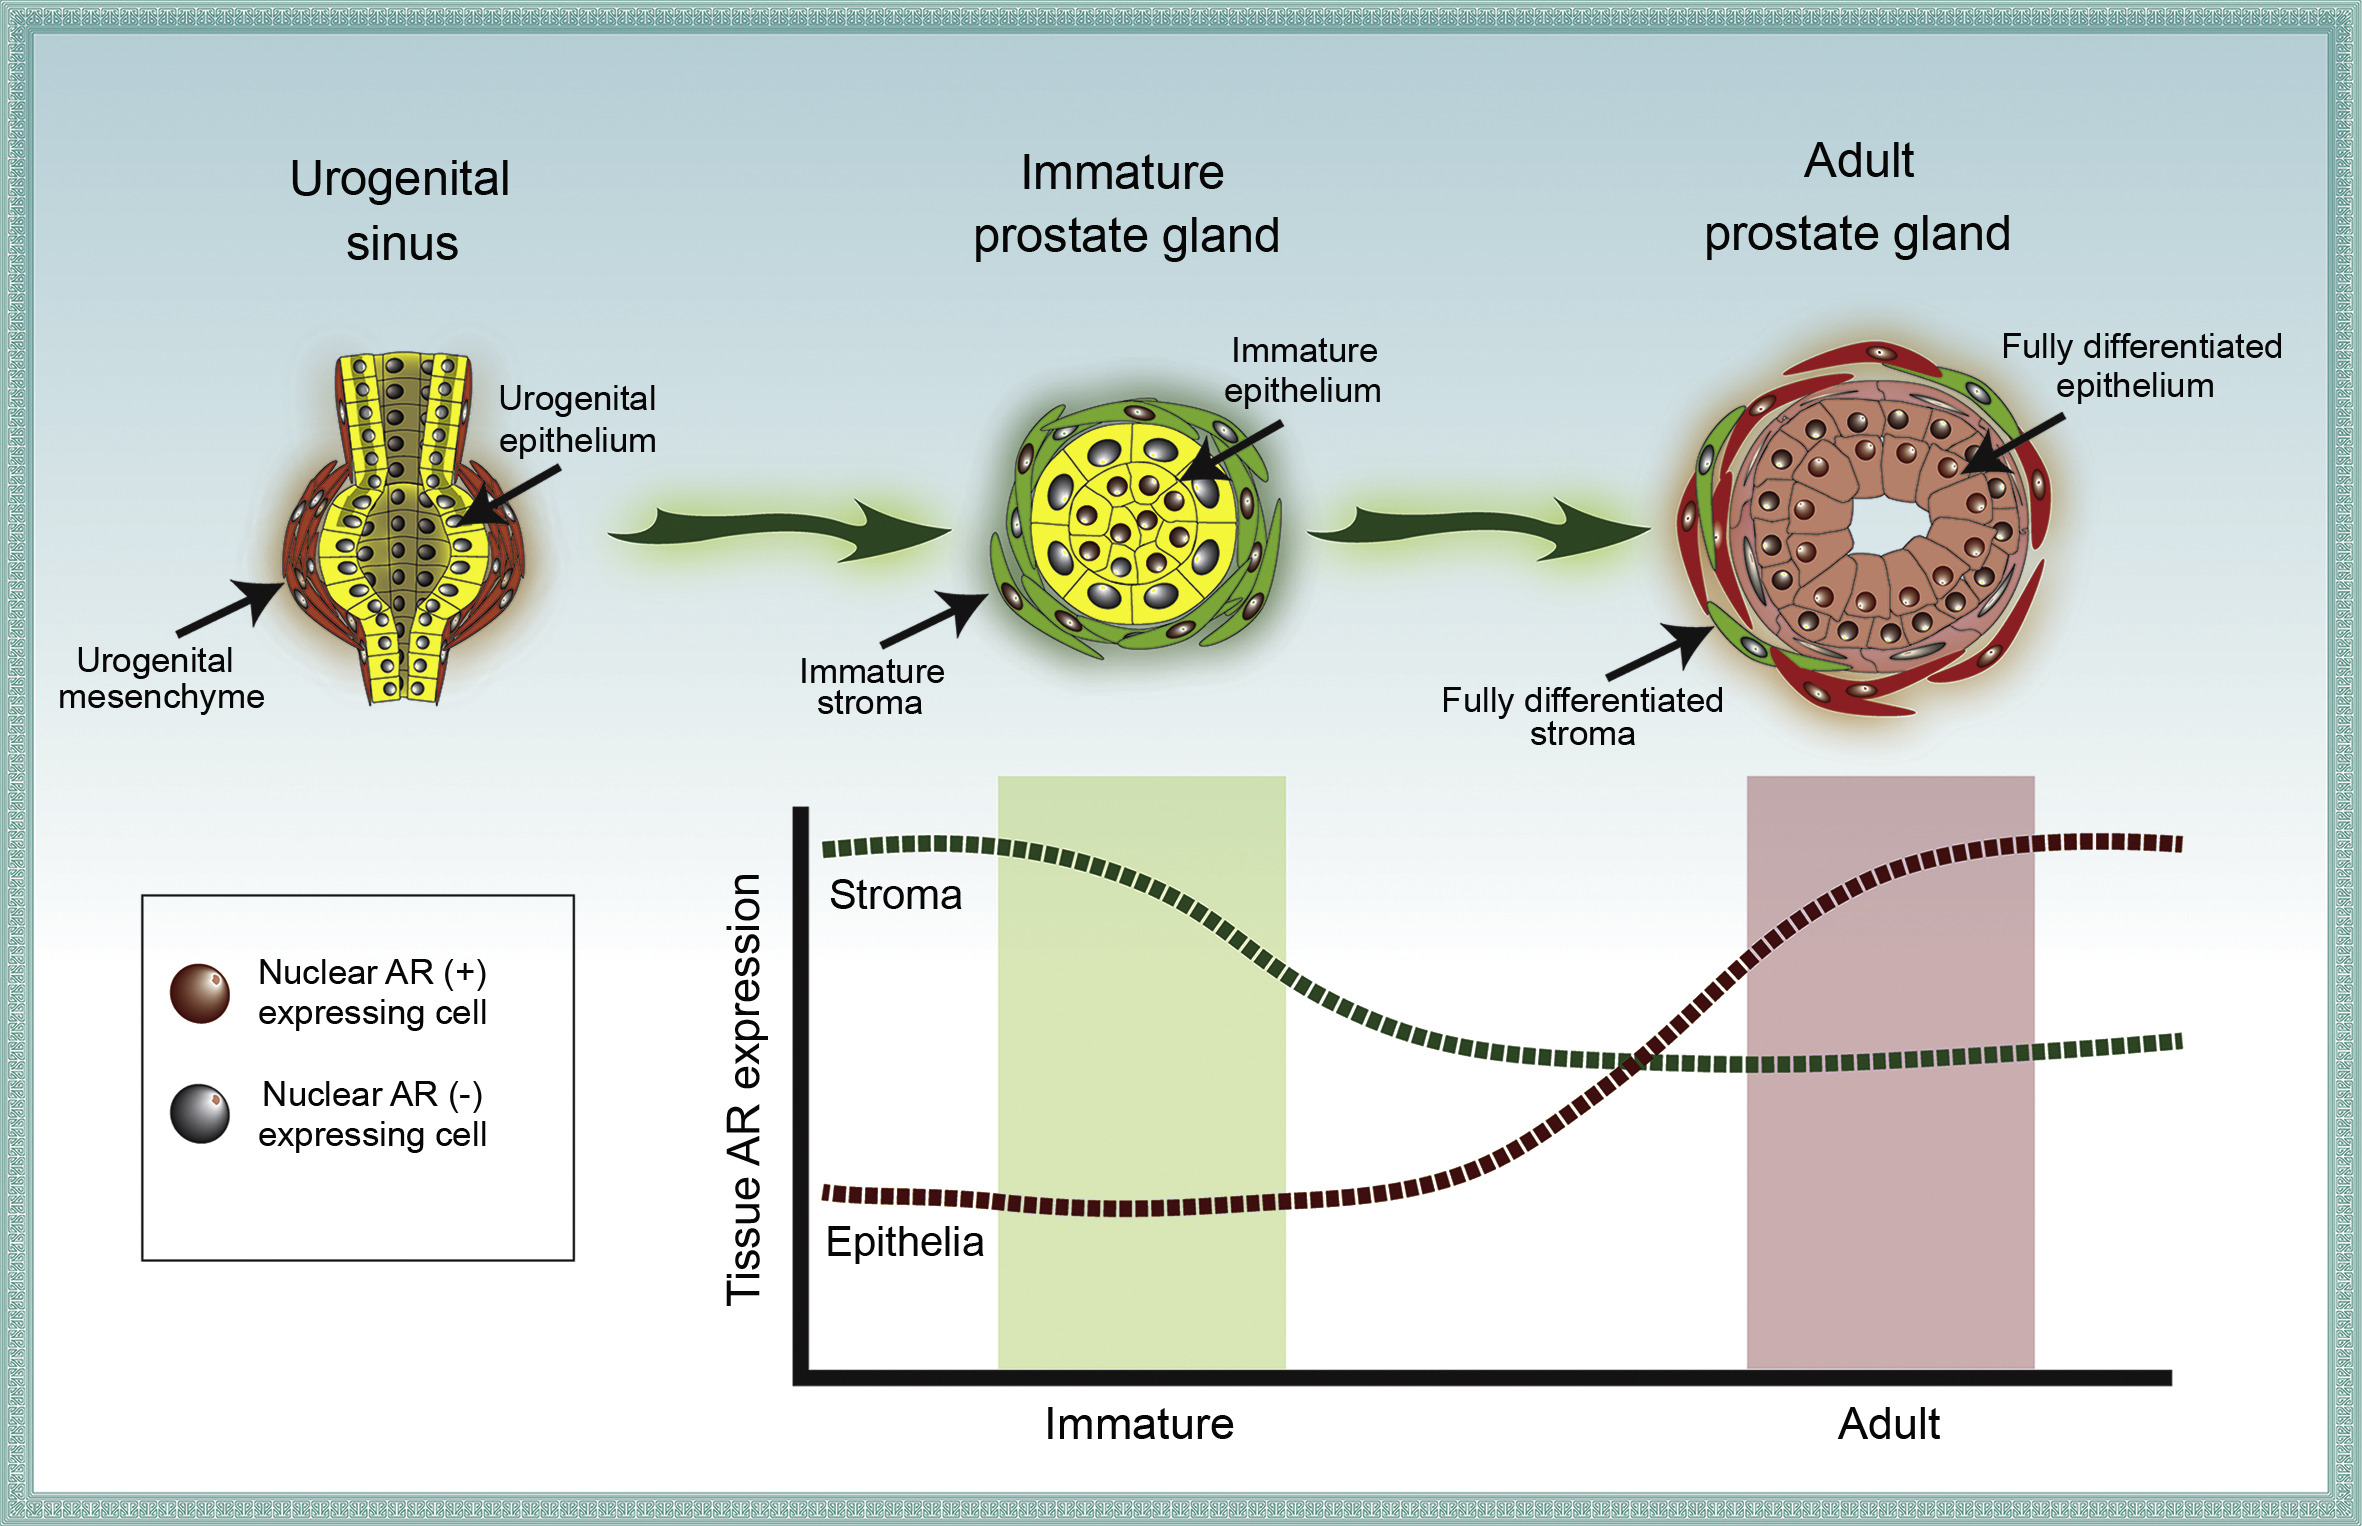
\includegraphics[keepaspectratio,width=\textwidth]{Introduction/Figures/prostatedevelopment.jpg}
        \caption[Development of the prostate]{\textbf{Development of the prostate} initiated by the development of the urogenital sinus (UGS), followed by extensions of prostatic buds to form an immature prostate gland. The adult prostate contains differentiated epithelial and stromal compartments. AR expression transitions from primarily stromal to epithelial during adult development. Figure reused under creative commons license \cite{Vickman2020Jul}}
        \label{prostatedevelopment}
    \end{center}
\end{figure}


\subsection{Prostate Cancer}
\subsubsection{Epidemiology}
PCa is the second most common cancer in men worldwide, accounting for 1 in every 14 cancer diagnoses and 15\% of all male cancers \cite{James2024Apr}, ranking second only to lung cancer in mortality rates \cite{BrayF}. Global incidence varies substantially (Figure \ref{prostatestatistics}), partly attributed to socioeconomic healthcare factors and the extent to which prostate-specific antigen (PSA) testing is used \cite{Culp2020Jan}. Consequently, the highest incidence rates occur in developed regions: Northern and Western Europe, Australia, New Zealand, North America, and Southern Africa (age-standardised rate of 35.5 per 100,000), whilst under-developed countries in regions such as sub-Saharan Africa, parts of South America and Eastern Europe rank the lowest in incidence rates (12.6 per 100,000) \cite{Nyame2020Jan}. Mortality outcomes are strongly influenced by the availability of screening and treatment; thus, regions with lower reported incidence frequently exhibit higher mortality rates, reflecting disparities in healthcare access rather than differences in underlying disease burden \cite{Nyame2020Jan}. Of note, elevated incidence of PCa in Caribbean and sub-Saharan African countries may be linked to genetic variants associated with PCa occurring more frequently in men with West African ancestry \cite{Culp2020Jan, Rebbeck2013Feb}. This is evident in North America, where African American men are twice as likely to contract the disease \cite{Brawley2012Sep}. In Asian countries, incidence and mortality rates are low (Figure \ref{prostatestatistics}); however, when Asian men migrate to the United States, their risk increases \cite{Kimura2012Sep}, indicating that low incidence and mortality rates in Asia are potentially due to a lack of population-based data across most of the countries in this region \cite{Baade2013Jun}.  In Ireland, approximately 4000 men are diagnosed with PCa annually, with 1 in 6 expected to contract the disease in their lifetime \cite{NCRI}. The overall five-year survival rates for Irish men diagnosed with PCa are 92.5\% for primary localised PCa \cite{NCRI}, reflecting advancements in effective treatment and earlier detection through increased testing of Irish men.

\begin{figure}
    \begin{center}
        %\includegraphics[angle=90,origin=c,width=\textwidth, height=0.7\textheight,keepaspectratio]{Figure1.png}
        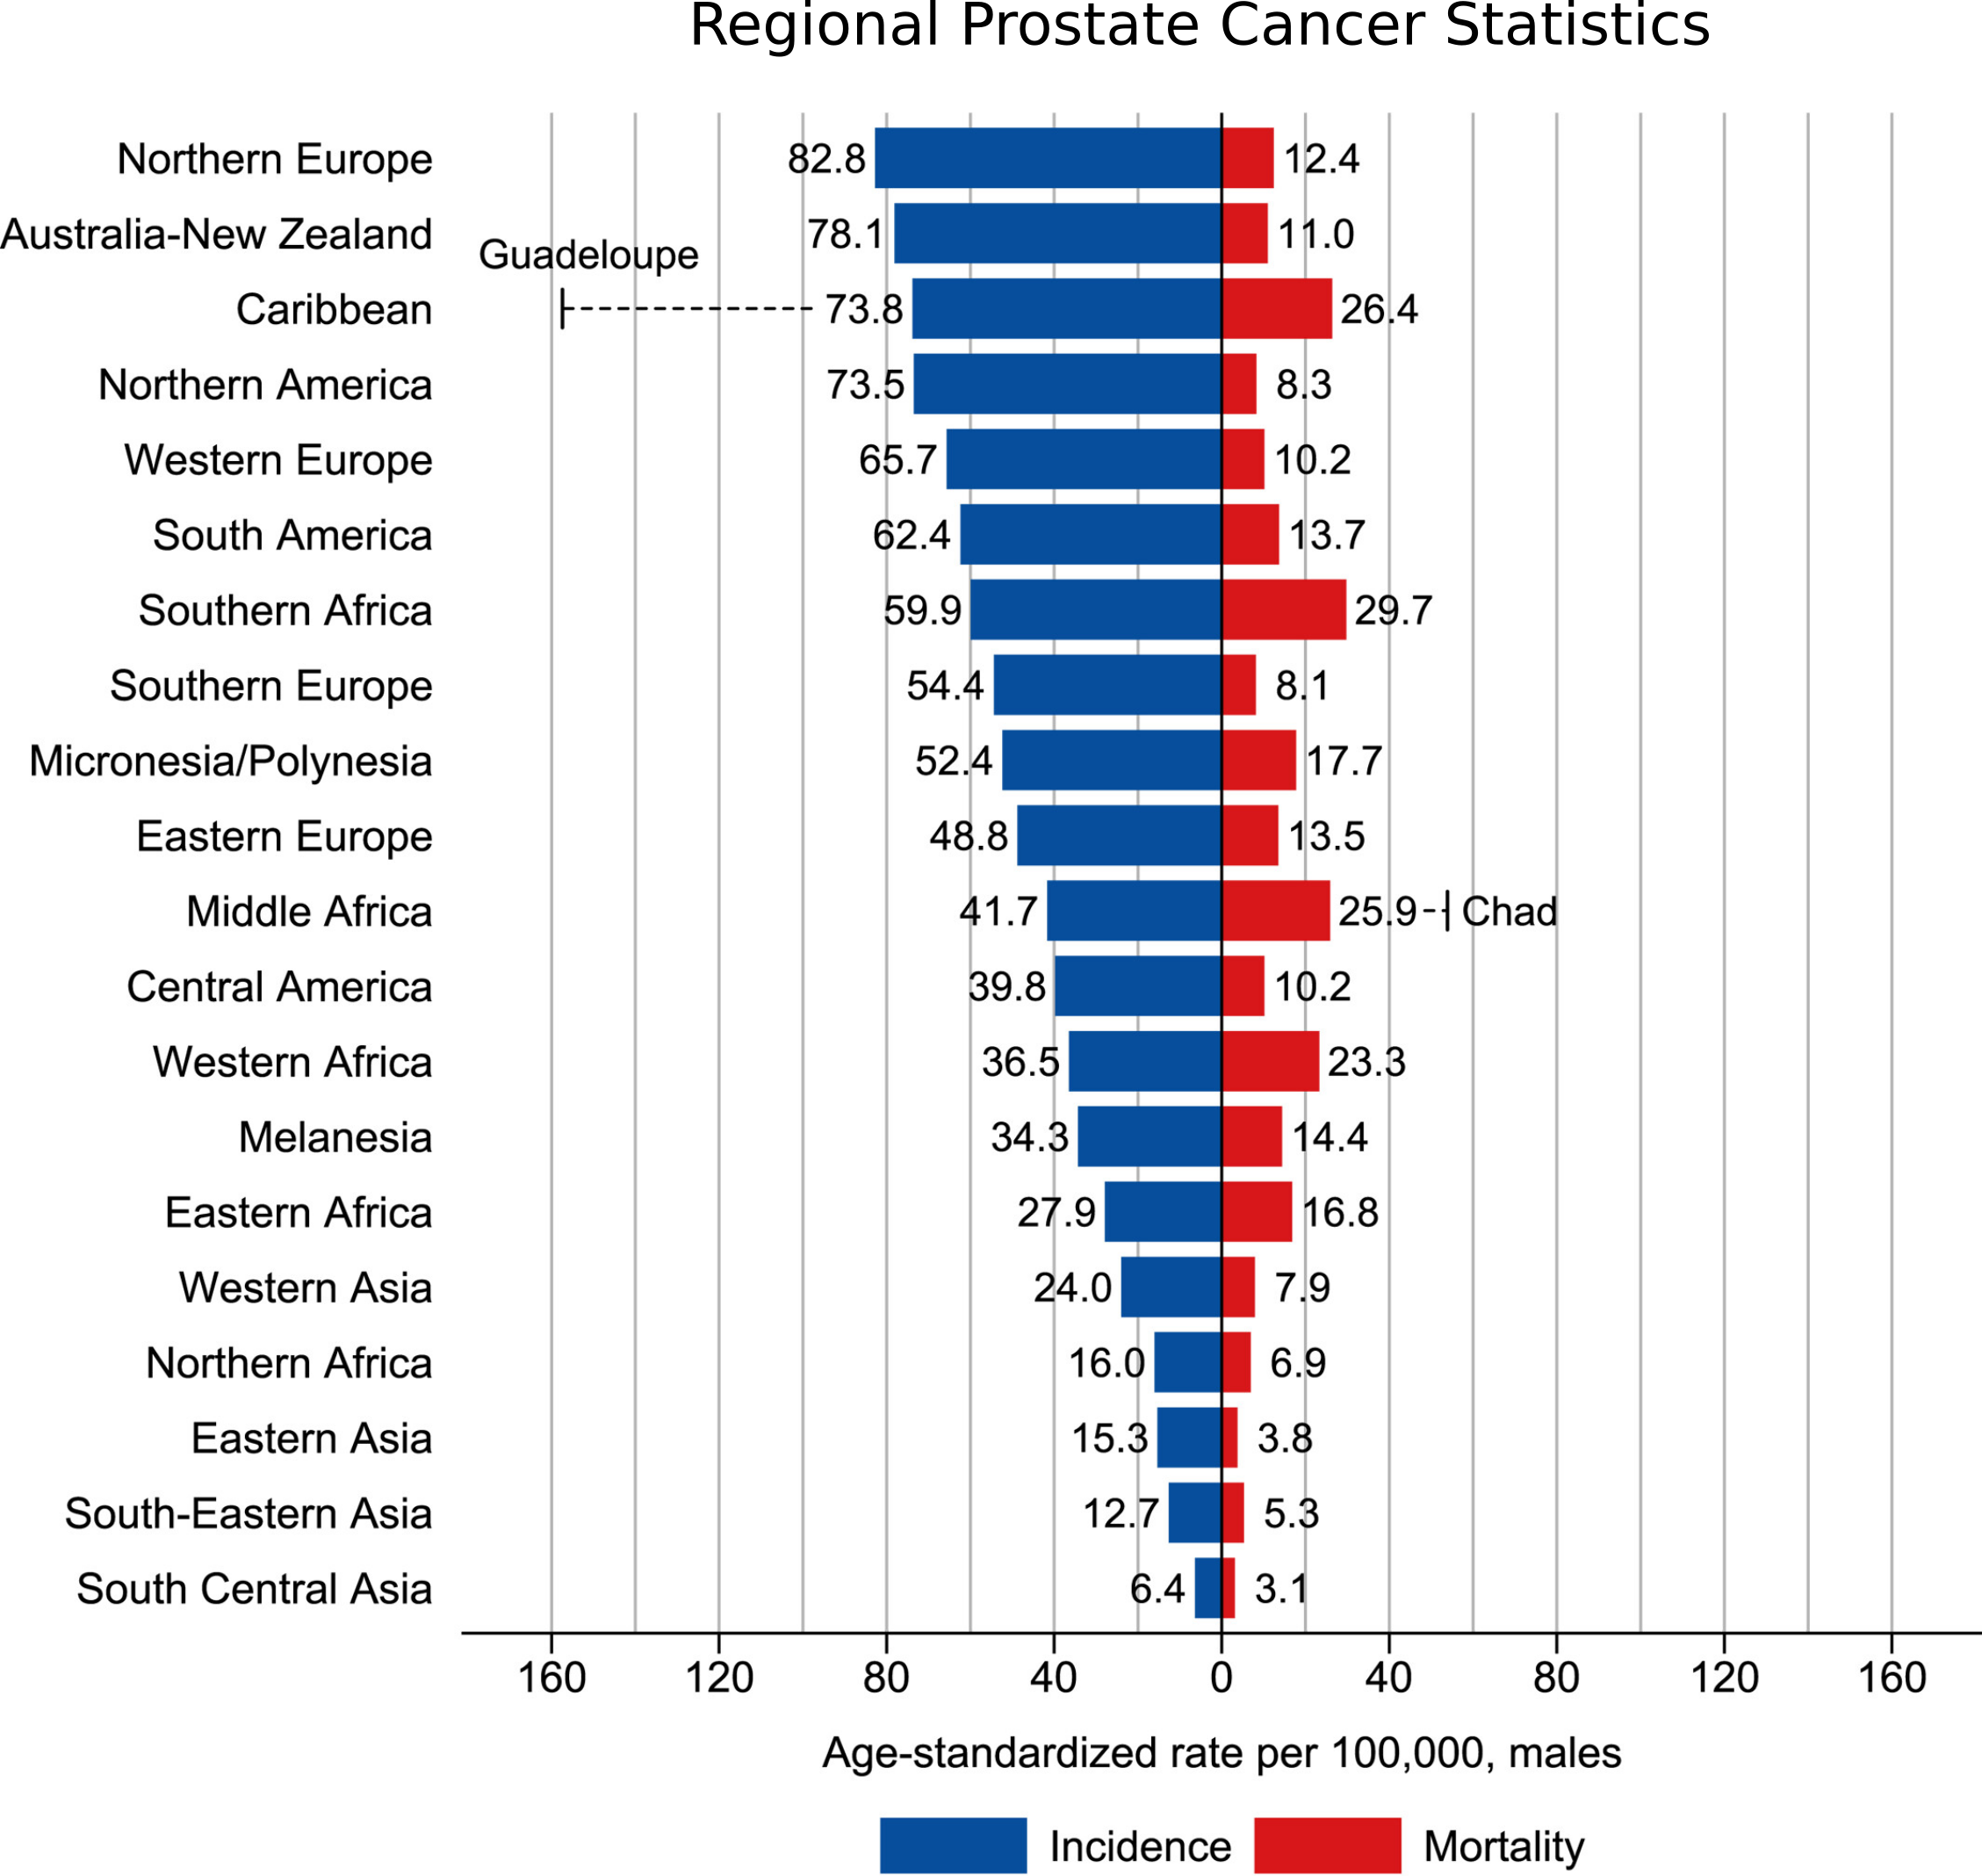
\includegraphics[keepaspectratio,width=\textwidth]{Introduction/Figures/prostatestatistics.png}
        \caption[Region-specific bar chart of prostate cancer incidence]{\textbf{Region-specific bar chart of prostate cancer incidence} and mortality age-standardised rates (GLOBCAN 2022). Permission granted for reuse from John Wiley and Sons under license number 5982410882196 \cite{Bray2024May}}
        \label{prostatestatistics}
    \end{center}
\end{figure}

\subsubsection{Aetiology}
Established risk factors for PCa include age, ethnicity, obesity and family history. Age-specific incidence rates and the aggressiveness of PCa rise after age 55 and peak at ages 70-74 \cite{Gann2002, Milonas2019Sep}. The population-based Surveillance, Epidemiology, and End Results (SEER) study reveals the 10-year risk of PCa increases from 2.3\% at age 50 to 7.3\% at 70. In addition, $\sim$60\% of men diagnosed with PCa are older than 65 \cite{SEER}. Epidemiological studies show African Americans are approximately 60\% more likely to develop PCa and exhibit nearly double the mortality rate when compared to white American males \cite{Gann2002}. It is unclear whether this stems from differences in socioeconomic status variables and access to healthcare or if there exists an inherent difference in the underlying PCa biology of both cohorts \cite{Tewari2005Dec}. As previously mentioned, men of West African descent harbour more genetic variants linked to PCa \cite{Culp2020Jan, Rebbeck2013Feb}; however, it is more likely that an interaction between genetic and environmental factors is responsible for increased PCa risk in African Americans. \par
The terms familial and hereditary PCa imply increased risk but are not analogous. Familial PCa is a result of cancer clustering within a family, often due to shared environmental factors, whilst hereditary PCa is genetic and is defined as a family with 1) three generations affected, 2) three first-degree relatives affected or 3) two relatives affected before age 55 \cite{Potter2000}. The pooled incidence rate ratio for men with an affected brother or father is 2.48 (95\% CI 2.25-2.74), with an affected brother yielding a higher rate ratio of 3.14 (2.37-4.15) than an affected father alone (2.35; 2.02-2.72), and the pooled estimate for two or more affected first-degree members is 4.39 (2.61-7.39). Strikingly, first-degree family history increases the incidence rate in men under 65 (RR:2.87, CI:2.21-3.74) compared to men over 65 with no familial history (1.92, 1.49-2.47) \cite{Kicinski2011Oct}. \par
Studies have revealed a positive correlation between high BMI and high-grade nonmetastatic and metastatic PCa \cite{Rodriguez2007Jan}. Furthermore, patients with a BMI $>$30 are at risk of developing metabolic syndrome (MetS), a cluster of cardiovascular risk factors including hypertriglyceridemia, central adiposity, hypertension, low HDL-C, and insulin resistance \cite{Grundy2004Jan}. MetS has been shown to harbour a positive association with pathologic Gleason score $>$8 and biochemical recurrence (BCR) of the disease \cite{Gacci2017Jun}. BCR is defined as PSA levels of $>$0.2ng/mL confirmed by a secondary measurement following undetectable PSA levels post-surgery \cite{Amling2001Apr}. However, levels exceeding $>$0.4ng/mL appear to more accurately predict the development of distant metastases \cite{Toussi2016Jun}.  

\subsubsection{Disease initiation}
PCa often exhibits high levels of interpatient heterogeneity (ethnic/geographical) and intrapatient heterogeneity. Cells within different tumour foci may arise from cellular ancestors that transformed independently or from a single transformed ancestor clone generating distinct clones and subclonal lineages \cite{Rebello2021Feb, Boyd2012Nov}. Consequently, the true cell of origin for all prostatic adenocarcinomas remains a contentious issue. PCa cells are thought to originate from basal or luminal prostatic epithelial cells, however, non-epithelial cells can also play a role in PCa initiation and progression \cite{Goldstein2010Jul, Chua2014Sep, Lee2015Dec}. Approximately 25\% of men in their 50s and up to 90\% in their 80s may present with abnormal, non-cancerous cell growth and proliferation of luminal epithelial cells in the transition zone, known as benign prostatic hyperplasia (BPH) \cite{Bushman2009Nov}; however, BPH is not considered to be a precursor for PCa cells, which by definition, must possess the capacity to invade the basement membrane to be classified as cancerous \cite{Kristal2010May}. \par 
In contrast to BHP, non-malignant lesions termed high-grade prostatic intraepithelial neoplasia (PIN) are frequently detected adjacent to PCa cells and are considered precursors to PCa \cite{Rebello2021Feb}. PIN occurs in the peripheral regions of the prostate gland and is characterised by intraglandular proliferation of luminal epithelial cells accompanied by compromised integrity of the basal cell layer \cite{Ayala2007Aug, Bostwick2004}. Morphologically, high-grade PIN cells display enlarged nuclei with prominent cytoplasmic basophilia and nucleoli \cite{Bostwick2004Mar}. A series of genomic alterations common to both high-grade PIN and PCa cells may serve as clues to PCa initiation: silencing of GSTP1 enzyme resulting in increased oxidative cell damage \cite{Lee1994Nov}, inactivation of tumour suppressor genes due to loss of heterozygosity on 8p12-21 detected in 63\% of PINs and 90.6\% of PCa cells \cite{Emmert-Buck1995Jul}, loss of \textit{NKX3-1} expression correlating to tumour progression \cite{Asatiani2005Feb} and amplification of \textit{ARNT} \cite{Kim2013Feb}. Jung et al. demonstrated that PCa genomes are direct descendants of high-grade PIN genomes \cite{Jung2016May}, postulating that high-grade PIN genomes require additional genomic modifications, such as \textit{TMPRSS2-ERG} fusions, to progress to PCa \cite{Fraser2017}. \par

\subsubsection{Screening and early detection}
Screening for PCa is the primary method for detecting localised PCa in asymptomatic men at a stage when the disease is potentially curable. Ideally, screening should be able to discriminate between tumours that require immediate action and definitive therapies with intent to cure from tumours that remain indolent and can be managed through active surveillance. The two main screening strategies for PCa are 1) a digital rectal exam (DRE) and 2) a PSA test. The former involves physical palpation of the prostate gland to assess its texture, checking for hard sections or nodules that may be cancerous, whilst the latter is a minimally invasive blood test assessing PSA levels. In men younger than 60, a PSA level of $<$2.5ng/mL is considered normal, while in men over 60, PSA levels $<$4.0ng/mL are considered non-elevated. Increased PSA levels occur naturally with age, however, increased PSA levels are also a marker of PCa due to malignant PCa cells lacking a structurally intact basal layer that otherwise restricts the extravasion of PSA to the prostatic ducts and bloodstream \cite{David2024Sep}. Thus, PSA screening has received negative attention in the literature, as elevated levels of PSA may be due to normal prostate cells or noncancerous conditions such as BPH or prostatitis, resulting in substantial risk of overdiagnosis and overtreatment of clinically indolent PCa \cite{JuliaHayes2014Mar, Ilic2013Jan}. A meta-analysis of published studies relating to the benefits of PSA screening substantiates this point: 570 men were needed for screening to prevent one death from PCa \cite{Tesfai2024May}. Despite this, the European Randomised Study of Screening for Prostate Cancer study (n=182,160) revealed a 20\% reduction in PCa-specific mortality over a follow-up of 16 years, demonstrating the ability of PSA screening to reduce PCa mortality at a population level \cite{Hugosson2019Jul}. \par
In the event of a high PSA reading, clinicians may pursue other avenues to determine if biopsy is necessary. Free PSA tests determine the ratio of PSA bound to antichymotrypsin (ACT) vs. the level of unbound PSA in a blood sample. Christensson et al. reported that PCa patients exhibit higher proportions of PSA-ACT than those with BPH \cite{Christensson1993Jul}, thus a result showing lower percentages of free PSA compared to PSA-ACT may warrant a biopsy. In patients presenting with high PSA levels and a negative biopsy, a molecular test to assess levels of mRNA from the prostate cancer antigen 3 (\textit{PCA3}) gene can be used to adjudicate if a repeat biopsy is required. Regardless of the chosen screening strategy, current guidelines recommend a multivariate approach accounting for factors such as age and family history to make an informed decision-making process for each patient \cite{Mottet2017Apr}.

\subsubsection{Diagnosis}
Pathways for PCa diagnosis when a DRE examination or PSA test results raise suspicion of PCa include sampling the prostate via transrectal ultrasound (TRUS) biopsy. TRUS-guided biopsies systematically sample 10-12 cores for histopathological evaluation, with a 30-40\% chance of detecting PCa in its first pass \cite{Ploussard2014Jan}. Drawbacks of TRUS biopsies include the risk of developing potentially life-threatening Gram-negative sepsis, estimated to be 3\% \cite{Loeb2013Dec}, bleeding, erectile dysfunction, and incomplete sampling of the prostate. By design, samples are taken from the peripheral zone bilaterally from the apex to the base of the gland, omitting parts of the anterior and caudal prostate. This strategy is of concern as the anterior apex has been found to frequently harbour cancerous cells, which when missed, require additional biopsies \cite{Moussa2010May}. More recently, the 3-Tesla multiparametric MRI (mpMRI) and an MRI-targeted transperineal biopsy have superseded the TRUS biopsy. mpMRI considers multiple parameters: 1) T1 and T2 anatomical imaging; 2) diffusion-weighted imaging (assessing the movement of water, known to be restricted in areas of cancer); and 3) contrast-enhanced imaging whereby the enhanced blood supply to cancerous cells takes up and releases the dye more quickly \cite{Moore2013Jan}. MRI results are assessed according to the Prostate Imaging Reporting and Data System (PI-RADS) on the scale of 1-5, with scores greater than or equal to 3 indicative of clinically significant prostate cancer, and a decision regarding biopsy is made \cite{Klotz2021Apr}. Transperineal biopsies carry a lower risk of infection (0.2\%) than transrectal biopsies, as the needle route bypasses the rectal wall, avoiding potential contamination. Nonetheless, the European Association of Urology (EAU) guidelines recommend combining targeted and systematic biopsies regardless of approach \cite{Chernysheva2026Sep}.

    \par
When establishing a diagnosis, each biopsy site is reported individually, including information on location, differentiation grade and extent. Differentiation grading may follow the Gleason scoring system or the International Society of Urological Pathology (ISUP) grading. The Gleason scoring system has been the standard for $>$40 years, in which microscopic evaluation of histological features within the tumour architecture is used to classify the tumour as poorly-differentiated (high grade) or well-differentiated (lower grade) \cite{Gleason1974Jan, Kweldam2019Jan}. The final Gleason score is the summation of the first and second most prominent Gleason pattern grades, with low ($<$6), intermediate (7) or high (8-10) comprising the final Gleason scores. In 2014, the Gleason scores were reorganised into ISUP grades 1-5, primarily to account for the differentiation of Gleason score 7, which may be composed of 3+4 or 4+3 observations (the predominant pattern is recorded first), in addition to the amalgamation of Gleason scores 9 and 10 to ISUP grade 5 \cite{Epstein2015Jul}. The World Health Organisation adopted the ISUP grading system in conjunction with PSA results and clinical T category (cT) to refine patient diagnoses further: patients are classified as low risk (cT1-cT2a, PCa $<$10ng/mL, ISUP grade 1), intermediate risk (cT2b or PSA $>$10-20ng/mL or ISUP grade 2) and high risk ($>$cT2b or PSA $>$20ng/mL or ISUP grade $>$3) \cite{Mottet2017Apr}.

\subsubsection{Disease progression}
PCa progresses in most patients, characterised by rising PSA levels suggestive of elevated AR activity owing to the proliferation of luminal epithelial cells. Early-stage PCa is androgen-dependent; therefore, traditional treatment strategies focus on attenuating the AR signalling pathway by blocking androgen binding to the AR, or via inhibition of transcriptional activity of the AR using androgen-deprivation therapy (ADT) or second-generation antiandrogens \cite{Li2025Feb}. These methods have been shown to greatly enhance progression-free survival rates of patients \cite{Fizazi2017Jul}, yet tumours may still arise from a subpopulation of cells that are resistant de novo or acquire resistance induced by AR antagonists, leading to a castrate-resistant prostate cancer (CRPC) phenotype. These resistant PCa cells re-activate AR signalling through a variety of mechanisms: AR gene amplification, AR mutations (Table \ref{ARmuts}), and AR splice variants such as \textit{AR-V7} \cite{Csizmarik2021Oct}. \par

\subsubsection{Management and Treatment}
Patients diagnosed with localised PCa have 3 options: expectant management, surgery and radiation. Expectant management does not involve a definitive treatment following diagnosis and is typically reserved for low-risk PCa. It can be classified as watchful waiting where symptoms are treated with palliative intent, or active surveillance involving PSA testing, DRE or biopsies with intent to cure patients who develop significant PCa disease \cite{Filson2015Jul}. Age is the primary factor guiding the choice of expectant management strategy, with the final decision typically being patient-led. Active surveillance is the preferred choice for younger men with low-risk PCa (Gleason $\leq$7) \cite{Chen2016Jun}. In the Prostate Testing for Cancer and Treatment (ProtecT) trial, 1643 men with localised PCa were randomised into active monitoring (n=545), surgery (n=553) or radiation (n=545). Whilst the number of men who experienced clinical progression of PCa (112 vs. 46 vs. 46) or experienced metastasis (33 vs. 13 vs. 16) at 120 months was roughly double for men in the active surveillance arm of the study, these results had no statistically significant bearing on overall mortality. Only 8 (1.5\%), 5 (0.9\%) and 4 (0.7\%) of men treated using active surveillance, surgery and radiation, respectively, died from PCa \cite{Hamdy2016Oct, Donovan2016Oct}. \par
For men presenting with Gleason score $>$7 and PSA 10-20ng/mL, surgery and radiation are the primary methods for treatment. The ProtecT trial showed no significant difference between surgery vs. radiation with respect to clinical progression, metastasis and overall survival. Yet, surgical and radiation treatments reduced the risk of clinical progression and metastasis when compared to active surveillance \cite{Hamdy2016Oct, Donovan2016Oct}. Whilst longer-range follow-up data is unavailable in this study, it stands to reason that fewer BCR and metastasis events could lead to improved long-term overall survival at the population level. Furthermore, for men treated with surgery, adjuvant radiation has been shown to reduce the occurrence of BCR in patients with pT3 tumours (HR=0.51, 95\% CI=0.37-0.70, P=$<$0.0001) compared to `wait-and-see' following surgery \cite{Wiegel2014Aug}. \par
Androgen deprivation therapy (ADT) agents remain the mainstay treatment for men with metastatic castrate resistant prostate cancer (mCRPC). ADT agents can act as luteinizing hormone-releasing hormone agonists/antagonists, reducing testosterone production by the testes, or as antiandrogens, preventing testosterone from binding to the AR. Alternatively, they can act as androgen synthesis inhibitors, blocking CYP17. The first ADT agent that showed prolonged survival among men with mCRPC was docetaxel \cite{Sartor2018Feb}. Two phase 3 trials demonstrated significant overall survival benefits of docetaxel vs. control HR=0.76, 95\% CI=0.62-0.94, P=0.009 and HR=0.8, 95\% CI=0.67-0.97, P=0.02 \cite{Petrylak2004Oct, Tannock2004Oct} however, patients assigned to docetaxel experienced fever, cardiovascular events, nausea and vomiting, metabolic disturbances and neurologic events at a higher rate than the control group \cite{Petrylak2004Oct}. Two new second-generation ADT agents, abiraterone and enzalutamide, differ in their actions in the androgen axis: abiraterone acetate inhibits androgen biosynthesis, whilst enzalutamide inhibits AR signalling by binding the AR receptor \cite{Litwin2017Jun}. Both have been shown to slow disease progression and improve overall survival, whether before or after treatment using the first-generation agent docetaxel \cite{deBono2011May, Ryan2013Jan, Scher2012Sep, Beer2014Jul}. \par
Advances in the integration of genomic testing into the diagnostic pathway may facilitate a tailored approach to an individual's specific tumour molecular biology; detecting aberrations in DNA repair genes of the AR can be used to rule out patients who are unlikely to respond to docetaxel, abiraterone or enzalutamide \cite{Mateo2015Oct}. Similarly, detection of the AR-V7 splice variant, which lacks the ligand-binding domain targeted by abiraterone and enzalutamide, has been associated with primary resistance to these agents \cite{Antonarakis2014Sep}. Incorporating these genomic markers into treatment selection may therefore help clinicians avoid ineffective therapies, sparing patients unnecessary toxicity and enabling more rapid transition to a treatment strategy likely to provide clinical benefit.


\paragraph{AR Amplification}
\noindent Clinically, AR amplification is significantly overrepresented in CRPC tumour samples that are refractory to ADT when compared to benign tissue or primary PCa tissue (Figure \ref{armutations}) \cite{Bubendorf1999Feb}, suggesting that CRPC cells undergo selective pressure to circumvent ADT intervention. Mechanistically, AR amplification increases AR expression, resulting in hypersensitivity to low levels of circulating androgens \cite{Waltering2009Oct}. A recent study has detailed a novel interaction between the overexpression of transcription factors MYB and AR, whereby MYB overexpression facilitates ligand-independent nuclear localisation of transcriptionally active AR, sustaining AR transcriptional activity under ADT conditions \cite{Srivastava2012Mar, Srivastava2021Nov}. Notably, AR amplification is more common in patients exhibiting biochemical recurrence after treatment using enzalutamide compared to abiraterone (58\% vs. 17\% P=0.02) \cite{Azad2015May}. Patients with AR gain in cell-free DNA have poorer progression-free survival (HR: 5.52, 95\% CI: 2.57-11.83, P $<$0.0001) and overall survival rates (HR: 12.06, 95\% CI: 4.94-29.49, P $<$0.0001) compared to normal AR status patients when treated with enzalutamide or abiraterone \cite{DelRe2021Jun}. AR amplification may be a useful biomarker for identifying candidates suited to treatment using second-generation ADT. \par

\paragraph{AR Mutations}
\noindent Similar to AR amplification, AR mutations confer a selective advantage for tumor cells in a low androgen environment resulting from hormone therapy. The first AR mutation identified was a missense mutation T877A, located in helix 11 of the AR LBD, which when mutated, showed robust AR transcriptional activity and could not be inhibited by the nonsteroidal antiandrogen bicalutamide \cite{Sun2006Jun}. The replacement of T877 by alanine facilitates promiscuous activity, where the mutant AR can bind to other hormones and analogs such as progestins, estrogens and cortisol. The binding of progesterone, estradiol or flutamide has been shown to activate AR-T877A \cite{Sack2001Apr}. Also located in the LBD, the mutation H874Y increases the size of the ligand-binding pocket, accommodating nonandrogenic steroid ligand activation by nilutamide \cite{Duff2005Dec}. Joseph et al. and Korpal et al. both report antagonist-to-agonist switching of the AR due to the point mutation to the LBD at F876L following patient treatment using enzalutamide \cite{Joseph2013Sep, Korpal2013Sep}. Overall, there is clear evidence that disease progression following ADT therapy can be facilitated by treatment-specific induced mutations to the AR, broadening the ligand specificity of the AR giving rise to a `mutator phenotype' \cite{Steinkamp2009Apr, Bielas2006Nov}. \par

\paragraph{AR Splice Variants}
\noindent Dehm et al. and Hu et al. identified AR splice variants producing a truncated AR protein which remains constitutively active in the absence of androgens \cite{Dehm2008Jul, Hu2009Jan}. AR splice variants are generated from transcribed intronic regions of intron 3, termed `cryptic exons' (CE1, CE2 and CE3) which, due to somatic nonsense mutations, splice a combination of cryptic exons to exon 3 of the AR, generating AR-V1 to AR-V7 splice variants \cite{Hu2009Jan}. Each of these AR variants produce premature termination codons downstream of the AR DBD, resulting in truncated ARs missing a LBD capable of evading nonsense-mediated decay \cite{Ajiboye2017Jun}. Regarding disease progression, elevated expression of AR-V7 is observed in CRW22 patient-derived xenographs refractory to abiraterone and enzalutamide \cite{Li2013Jan, Zhu2020Nov}. \par

Irrespective of the underlying genomic abberations, most patients will acquire resistance to ADT, progressing to CRPC and ultimately metastatic CRPC, which carries a far worse prognosis. Therefore, it is of utmost importance to investigate biomarkers associated with disease progression to effectively stratify patients, identify novel targets and develop personalised treatment strategies for patients. 

\begin{figure}
    \begin{center}
        %\includegraphics[angle=90,origin=c,width=\textwidth, height=0.7\textheight,keepaspectratio]{Figure1.png}
        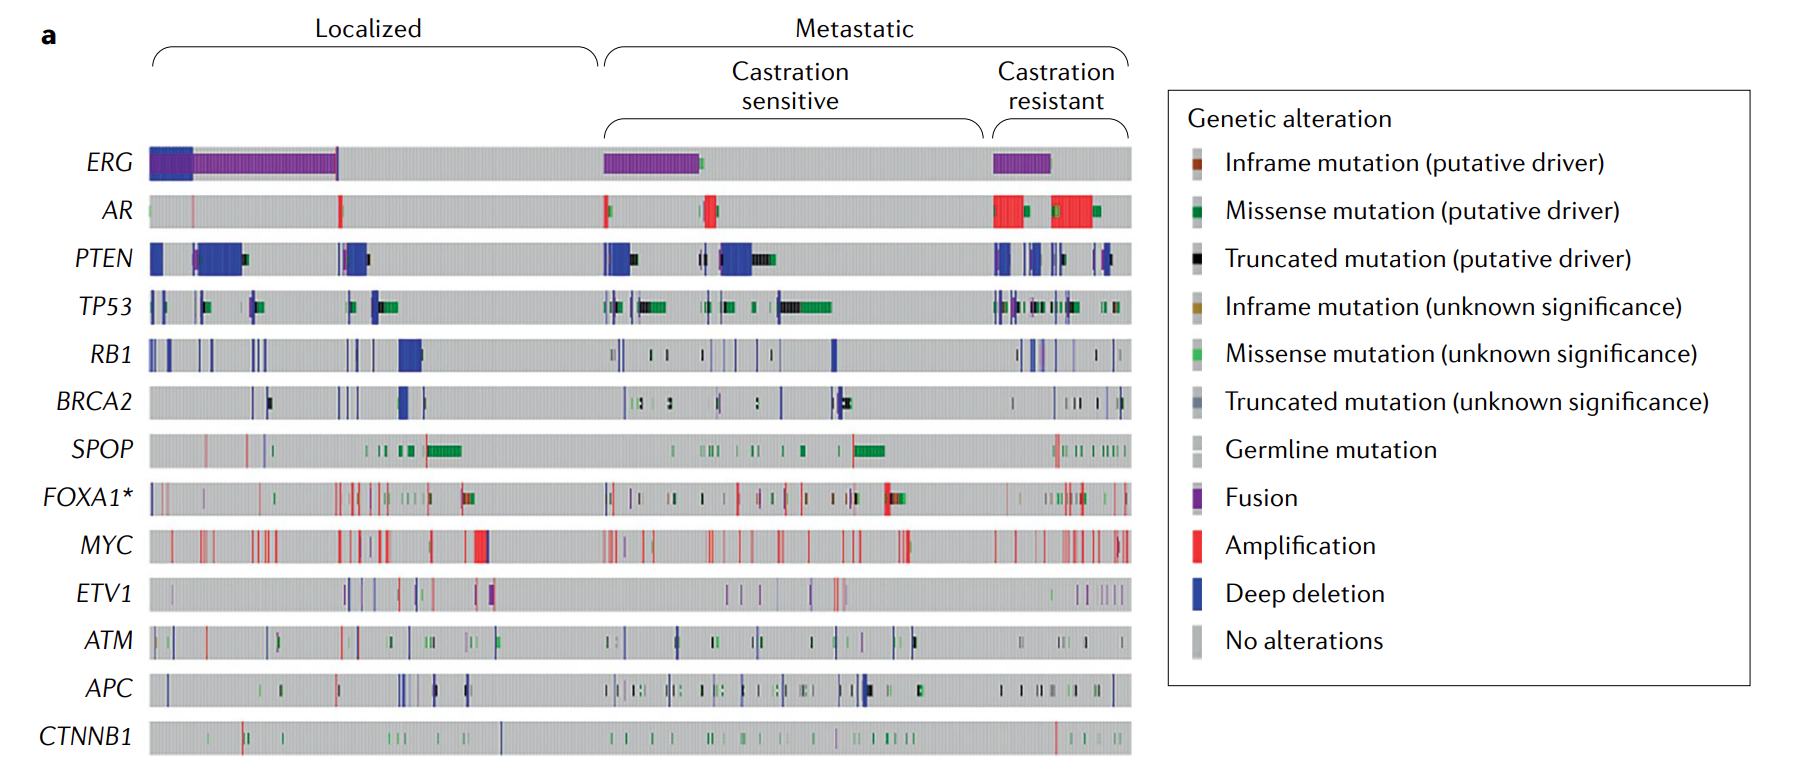
\includegraphics[keepaspectratio,width=\textwidth]{Introduction/Figures/AR_mutations.png}
        \caption[Genetic alterations in prostate cancers]{\textbf{Genetic alterations in prostate cancers}: localized, metastatic castration-sensitive prostate cancer (mCSPC) and metastatic castration-resistant prostate cancer (mCRPC) (localized, 494 samples; mCSPC, 424 samples; mCRPC, 150 samples). Permission granted for reuse from Nature Reviews Disease Primers under license number 5996481096401 \cite{Rebello2021Feb} }
        \label{armutations}
    \end{center}
\end{figure}

\iffalse
Cancer-associated fibroblasts (CAFs) are abundantly present in the prostate tumour microenvironment (TME), with reduced AR expression in CAFs considered a prognostic factor of PCa progression, suggesting CAFs may act as a negative regulator of PCa development \cite{Tang2021Oct}. Palethorpe et al. demonstrated \textit{in vitro} AR activation in human prostate myofibroblasts retarded growth of multiple PCa cell lines (PC3, Du145, C4-2B, LNCaP) \cite{Palethorpe2018Apr} whilst Cioni et al. showed loss of AR in CAFs downregulated \textit{CCL2} and \textit{CXCL8} cytokine expression, facilitating PCa cell migration \cite{Cioni2018Aug}. Second-generation therapies such as enzalutamide inhibit AR-mediated PCa growth, but consequently elevate metastasis-related markers N-cadherin \cite{Jennbacken2010Jun}, Cadherin-11 \cite{Lee2010May, Chu2008Aug} and nestin \cite{Kleeberger2007Oct}. In a phase II study, abiraterone was shown to successfully reduce PSA levels by 50\% or more in 79\% of patients, yet 43.5\% of patients experienced bone scan flare lesions indicative of bone metastases \cite{Ryan2011Jun}. 
\fi

\renewcommand{\arraystretch}{1.4}
\begin{table*}[h!]
\caption[Summary of selected androgen receptor mutations]{\textbf{Summary of selected androgen receptor mutations}. LBD: Ligand-binding domain; Nterm: amino-terminal domain. Full mutation catalogue available at \href{https://androgendb.mcgill.ca/}{https://androgendb.mcgill.ca/} \cite{Gottlieb2012May}.\label{ARmuts}}
\resizebox{\textwidth}{!}{%
\begin{tabular}{llcp{9cm}r}
\toprule
\textbf{Mutation} & \textbf{Position} & \textbf{Exon} & \textbf{Description} & \textbf{Reference} \\
\midrule
Substitution & L701H   & 4/LBD  & Reported in hormone-refractory PCa patients. Highly responsive to AR activation via circulating ligands, cortisol and cortisone. & \cite{vandeWijngaart2009Dec} \\
Substitution & T877A   & 8/LBD  & Exhibits robust AR activity in the presence of antiandrogens. & \cite{Sun2006Jun, Chen2004Jan} \\
Substitution & W741C   & 5/LBD  & Bicalutamide-liganded W741C mutant AR coactivated by $\beta$-catenin. & \cite{Masiello2004Oct} \\
Deletion     & CAG-repeats & 1/Nterm & Shorter repeats correlate with younger diagnosis, higher grade and higher stage PCa. & \cite{Bratt1999Oct} \\
Substitution & F876L   & 8/LBD  & Abolishes antagonistic activity of enzalutamide. & \cite{Joseph2013Sep, Korpal2013Sep} \\
\bottomrule
\end{tabular}%
}
\end{table*}

\subsection{Biomarkers in prostate cancer}
Detection of early stage PCa relies on PSA testing and a DRE, whilst localised advanced PCa can benefit from biopsy tests to establish cancer stage. In an effort to address the transitional stages of PCa progression, several biomarker tests have been developed to date. The prostate health index (PHI) attempts to increase the diagnostic value of PSA by combining total PSA, \% free PSA and [-2]pro-PSA to produce a scoring system \cite{Le2010Apr}. Intended as a diagnostic tool, its recommended use is for patients presenting with PSA levels between 2.0ng/mL and 10ng/mL. The PHI score outperformed each of its constituent parts (0.74 AUC (PHI), 0.72 \%[-2]proPSA, 0.63 [-2]proPSA, 0.61, \%free PSA and 0.56 total PSA) \cite{Stephan2013Jan}. For the diagnosis of advanced PCA, the 4K score was developed combining four different kallikrein markers (total PSA, \%free PSA, intact PSA, human-kallikrien-2 (hK2)), patient age and DRE results \cite{Vickers2010May}. Nordstrom et al. combined the 4K and PHI scoring systems in a study on 513 men with PSA levels ranging from 3.0 - 13.0ng/mL \cite{Nordstrom2015Jul}. Whilst AUC results from the 4K and PHI test were indistinguishable in detecting PCa of any form and advanced PCa, the authors used cut-off values (10\% 4K score, 39 PHI score) to stratify patients effectively. Results of the study demonstrated 29\% of unnecessary biopsies could be spared, however, 10\% of high-grade PCa cases would be missed using the cut-off points. \par
\subsubsection{Messenger RNAs
}
In 2015, the first genetic diagnostic test was developed termed SelectMDx, comprising a two gene panel (\textit{DLX1} and \textit{HOXC6}) PSA, age, history of prostate biopsy and family history \cite{Leyten2015Jul}. It has been shown that the use of SelectMDx in patients with PSA levels $>$3 ng/mL can reduce overdiagnosis and overtreatment and ultimately reduce total costs per patient and increase health-related quality of life \cite{Dijkstra2017Nov}. A secondary panel developed by MDx Health termed ConfirmMDx focuses on epigenetic changes in \textit{GSTP1}, \textit{APC} and \textit{RASSF1} genes in an effort to detect the `halo effect' surrounding tumor foci with abberations to any gene constituting a positive result \cite{Partin2014Apr}. As ConfirmMDx is predecated on detecting cancer, it cannot be used as a tool to rule out clinically significant PCa \cite{Leapman2016Feb}. As such, its recommendation is towards men before repeat biopsy following an initial negative biopsy \cite{Kretschmer2017Dec}. \par
Concerning prognostic tests for PCa, the Oncotype DX Genomic Prostate Score (GPS) assay evaluates 12 cancer-related genes and 5 reference genes to produce a score between 0-100, with 40 being the cut-off point for high-risk disease \cite{Klein2014Sep, Cullen2020Sep}. The Prolaris test, based on work by Cuzick et al. \cite{Cuzick2011Mar} evaluates 31 genes involved in cell cycle progression (CCP) creating a risk score effectively stratifying patients into $\leq$0, $>$0 to $\leq$1, 1 to $\leq$2 and $>$2 CPP score. An increase by one unit of the CCP score was able to independently predict BCR (HR=1.77, 95\% CI=1.40–2.22, P=$<$0.0001). The CCP was also able to significantly predict overall survival (HR=2.57, 95\% CI=1.93–3.43, P=$<$0.0001) \cite{Cuzick2011Mar}. The ProMark test utilises 12 proteomic biomarkers as a prognostic tool to detect aggressive PCa and lethal PCa \cite{Shipitsin2014a, Shipitsin2014b}. In a clinical validation study, the panel was refined to 8 proteomic signatures and using a cut-off score of $\leq$0.33, the authors found positive results in distinguishing low favourable vs. favourable pathology results (AUC 87.2\%) \cite{Blume-Jensen2015Jun}. Finally, the Decipher 22-gene panel based on genes involved in cell proliferation, androgen signalling, immune system modulation, cell cycle progression and cell structure, is primarily used to predict systemic progression of PCa following definitive therapy. The scoring system falls between 0-1, with values $>$0.6 considered high risk for progression \cite{Nakagawa2008May}. In an external evaluation study, Decipher was used to stratify patients into low risk $>$0.4, intermediate risk 0.4-$>$0.6 and high risk $>$0.6, effectively predicting freedom from BCR (0.78 AUC) and metastasis (0.80 AUC) in a cohort of 139 patients who recieved adjuvant or salvage radiotherapy following radical prostectomy \cite{Den2014Aug}. \par
A report from the International Society of Urological Pathology (ISUP) commented that genomic classifiers may provide utility in predicting disease progression under an active surveillance or postradical prostatectomy setting, if the tumor focus harboring the disease is adequately sampled. In addition, the report recommended further studies to assess the performance of the genomic signatures in relation to the heterogeneity inherent to needle biopsy samples, and to provide recommendations for sampling (which biopsy to use, multiple sampling from the same or different tumor foci) \cite{Lotan2020Jul}. Given that current PCa mRNA biomarkers are not a panacea, the research community must continue to search for new biomarkers that can aid in early diagnosis and prognosis of the patient as well as predict patient response to treatments. One such avenue is exploring non-coding RNAs involved in the competing endogenous RNA network, in which circular RNAs, microRNAs and messenger RNAs form a regulatory network capable of influencing gene expression in both normal and disease-based settings. 

\subsubsection{Micro RNAs}
Micro RNAs (miRNAs) are small 18-24 nucleotide non-coding RNAs that regulate the transcription of mRNAs by binding to complementary sequences in target mRNA, consequently blocking mRNA transcription or promoting degradation of the transcript \cite{Valencia-Sanchez2006Mar}. miRNAs can be found in several bodily fluids, including blood, urine, semen, and saliva, among others, exhibiting tissue-specific expression and dysregulation in cancer \cite{Weber2010Nov, Lin2015Jun}. Furthermore, miRNAs can be accurately quantified using techniques such as qRT-PCR, microarrays and small RNA sequencing, making them ideal candidates as biomarkers \cite{Fabris2016Aug}. \par
In PCa, miRNAs play important mechanistic roles, including inhibiting apoptosis, promoting cell proliferation, epithelial to mesenchymal transition (EMT) and growth under androgen-independent settings \cite{Bryant2012Feb} (Table \ref{PCamiRNAs}). Several studies have investigated the role of miRNAs as biomarkers in PCa, finding differentially expressed miRNAs according to PSA level, Gleason score and treatment using docetaxel \cite{Endzelins2017Nov, Mitchell2008Jul, Lin2014May}. Matin et al. demonstrated the diagnostic value of miR-4289, miR-326, miR-152-3p and miR-98-5p in differentiating PCa patients and healthy controls (AUC 0.88) \cite{Matin2018Apr}, whilst Sharova et al utilised miR-106a, miR-130b and miR-223 to distinguish localised PCa vs. BHP (AUC 0.84 vs. PSA only; AUC 0.56), aiding clinical decision making and avoiding unnecessary biopsies \cite{Sharova2016Jun}. \par
In addition to evaluating standalone miRNA signatures, researchers have begun constructing miRNA-mRNA bipartite networks composed of differentially expressed RNAs and predicted miRNA-mRNA pairs exhibiting inverse expression to model the regulatory effects of miRNAs \cite{Naghizadeh2023Jul, Lin2018Dec, Zhang2014Dec}. This `knowledge-based filtering' method has the potential to reveal miRNAs and mRNAs associated with cancers that may otherwise be omitted using traditional machine learning feature selection techniques. 


\begin{table*}[h!]
\centering
\caption[miRNAs upregulated in PCa]{\textbf{miRNAs upregulated in PCa}}
\resizebox{\textwidth}{!}{%
    \begin{tblr}{%
        colspec = {lX[2.5]r} %% put weights for column width in []
        }
        \hline
        \textbf{miRNA} & \textbf{Function} & \textbf{Reference} \\
        \hline
        miR-1290 & Promotes cell proliferation, migration and EMT transition & \cite{Li2022Jun} \\
        miR-141 & Overexpression inhibits SHP, promoting AR activity & \cite{Xiao2012Oct} \\
        miR-143 & Suppresses KRAS expression, regulates EMT transition & \cite{Ngalame2014Apr} \\
        miR-181 & Inhibits negative regulator of androgen receptor DAX-1 &  \cite{Tong2014Oct} \\
        miR-18a & OncomiR targeting tumor suppressor STK4 & \cite{Hsu2014Apr} \\
        miR-20 & Overexpression of miR-20 oncomiR attenuates pro-apoptotic E2F1–3 genes & \cite{Sylvestre2007Jan} \\
        miR-21 & Inhibits apoptosis by targeting PTEN, PDCD4 and promotes androgen-independant growth & \cite{Ribas2009, Yang2010Oct, Lu2008Jul} \\
        miR-221 & Stimulates androgen independent cell growth in LNCaP & \cite{Sun2014May} \\
        miR-375 & Acts as oncomiR in PCa progression, degrades CCND2 & \cite{Costa-Pinheiro2015Dec} \\
        miR-96 & Inhibits apoptosis, cell cycle arrest inducer FOXO1 & \cite{Ma2014Aug, Haflidadottir2013Aug} \\
        \hline
    \end{tblr}%
}
\label{PCamiRNAs}
\end{table*}

\subsubsection{Circular RNAs}
Circular RNAs (circRNAs) are a class of long non-coding RNAs generated via back-splicing of exons during alternative splicing of linear transcripts, producing a covalently closed loop structure resistant to exonuclease degradation \cite{Salzman2012}. circRNAs exhibit approximately a 2.5 times longer half-life than linear RNAs and up to 6 times longer half-life when encapsulated in exosomes \cite{Li2015Aug}, making them remarkably stable biomarkers. Similar to miRNAs, circRNAs can be found in bodily fluids and are detectable using high-throughput sequencing technologies for detection and quantification. \par
Several circRNAs are dysregulated in PCa (Table \ref{PCacircRNAs}) and associated with multiple stages of the disease. CircPDHX is associated with Gleason score, pathological T and overall survival in PCa, and facilitates the proliferation and invasion of PCa cells by sponging miR-378a-3p \cite{Mao2021Jan}. hsa\_circ\_0001165 and hsa\_circ\_0001085 play a regulatory role in the epithelial-mesenchymal transition of PCa cells via miR-187-3p and may indirectly regulate the PI3K-Akt signalling and TGF-$\beta$ signalling pathways through miR-196b-5p \cite{Yan2020Feb}. Lim et al. revealed upregulation of hsa\_circ\_0001275 and its parental gene \textit{PLCL2} in enzalutamide-resistant LNCaP clones \cite{Lim2021Dec}. \par
Whilst there exist multiple studies identifying dysregulated circRNAs in PCa, there is a dearth of statistical models published using circRNA expression data for prediction/classification tasks in PCa. Firstly, the number of total RNA-Seq datasets on PCa patients with suitable power for developing statistical models is scarce, and secondly, circRNAs are lowly expressed in cells compared to linear or miRNAs, making accurate quantification and zero-inflated counts an active challenge in the field. Despite their promise as a biomarker in PCa, there doesn't exist a gold-standard workflow for the accurate preparation and computational quantification of circRNAs to facilitate widespread use of predictive models using circRNAs. 

\begin{adjustwidth}{-1cm}{-1cm}
\footnotesize
    \begin{longtblr}[%
        entry = {circRNAs dysregulated in prostate cancer},
        caption = {\textbf{circRNAs dysregulated in prostate cancer}},
        label = {PCacircRNAs}
        ]{%
        width = \linewidth,
        colspec = {lX[1]X[0.7]X[2]r} %% put weights for column width in []
        }
        \hline
        \textbf{circRNA} & \textbf{CircBase ID} & \textbf{miR target} & \textbf{Function} & \textbf{Reference} \\
        \hline
        circSMARCA5 & hsa\_circ\_0001445 & - & Promotes cell proliferation, inhibits apoptosis & \cite{Kong2017Nov} \\
        circRNA-MYLK & hsa\_circ\_0141940 & miR-29a & Promotes cell proliferation, invasion and migration & \cite{Dai2018} \\
        circCSNK1G3 & hsa\_circ\_0001522 & miR-181b & Promotes cell migration & \cite{Chen2019Feb} \\
        circABCC4 & hsa\_circ\_0030586 & miR-1182 & Promotes cell proliferation & \cite{Huang2020} \\
        circAGO2 & hsa\_circ\_0135889 & - & Promotes cell proliferation, invasion and metastasis & \cite{Chen2019Jul} \\
        circHIPK3 & hsa\_circ\_0000284 & miR-193a-3p, miR-338-3p & Promotes cell migration and invasion & \cite{Chen2019FebII, Cai2019May} \\
        circZNF609 & hsa\_circ\_0000615 & miR-186-5p & Promotes cell proliferation and metastasis & \cite{Jin2019Dec} \\
        circ\_CCNB2 & hsa\_circ\_0035483 & miR-30b-5p & Promotes cell proliferation, autophagy, inhibits apoptosis & \cite{Cai2022Jul} \\
        circFOXO3 & hsa\_circ\_0006404 & miR-29a-3p & Promotes cell proliferation, inhibits apoptosis & \cite{Kong2020Jan} \\
        circ\_SLC19A1 & hsa\_circ\_0062019 & miR-497 & Promotes cell growth and proliferation & \cite{Zheng2020Apr} \\
        circSMARCA5 & hsa\_circ\_0071043 & miR-432 & Promotes cell glycolysis & \cite{Dong2021Feb} \\
        circDDX17 & hsa\_circ\_0063308 & miR-346 & Inhibits cell proliferation, invasion, and EMT & \cite{Lin2020Aug} \\
        circCRKL & hsa\_circ\_0001206 & miR-141 & Inhibits cell cycle, migration and invasion & \cite{Nan2020Nov} \\
        hsa\_circ\_0007494 & hsa\_circ\_0007494 & miR-616 & Inhibits cell migration and invasion & \cite{Zhang2020Oct} \\
        \hline
    \end{longtblr}
\end{adjustwidth}


\subsection{Thesis Outline}
The overarching aim of this thesis was to address current computational limitations in circRNA analysis and to characterise the regulatory role of circRNAs in prostate cancer. Specifically, we asked whether existing computational workflows could reliably detect, quantify and annotate circRNAs from short-read sequencing data, given the conflicting approaches adopted by current tools and databases. Given that no single existing resource or workflow adequately addressed these limitations, we then asked what tools could be built to fill this gap. Chapters 2–4 specifically address this research question, culminating in the development of nf-core/circrna and pycircdb. In our final research question, described in Chapter 5, we asked whether circRNAs, acting within the competing endogenous RNA network alongside miRNAs and mRNAs, contribute towards biochemical recurrence in prostate cancer, and whether this signal could be used to derive a prognostic gene set. 

In Chapter Two, we review the strengths, weaknesses and underlying assumptions of current computational methods for characterising circRNAs in sequencing data. Given that circRNAs represent only 1\% of the transcriptome pool compared to poly(A) RNA molecules, sufficient library preparation protocols and the mitigation of sequencing artefacts remain paramount for reducing false-positive circRNA calls. Next, we describe popular quantification tools utilising segmented-based and pseudo-reference-based approaches to detecting circRNAs using short-read sequencing reads. Given the disparate nature of these quantification tools, we provide a review of increasingly popular integration-based circRNA identification methods, whereby users define a set of filtering parameters to arrive at a set of high-confidence, consensus-based circRNAs.

In Chapter Three, we provide an overview of our novel integration-based circRNA quantification pipeline `nf-core/circrna: a portable workflow for the quantification, miRNA target prediction and differential expression analysis of circular RNAs'. Developed using nextflow, nf-core/circrna reduces the barrier to entry for researchers by providing an easy-to-use, platform-independent and scalable workflow for circRNA analyses. As part of the nf-core suite, nf-core/circrna adheres to standardised guidelines encompassing continuous integration testing, containerisation, and peer review, ensuring portability and reproducibility across computing environments \cite{Ewels2020Mar}.

Chapter Four seeks to address the limitations of current circRNA databases discussed in Chapter Two and extend the functionality of nf-core/circrna with our Python package `pycircdb: integrated circRNA database annotation for computational workflows'. In brief, pycircdb provides rapid, command-line access to multiple publicly available circRNA databases, addressing the ambiguous nomenclature and absence of programmatic interfaces that currently limit their utility. 

Chapter Five examines the role of the competing endogenous RNA network, consisting of circRNAs, miRNAs and mRNAs, in prostate cancer. For each RNA biotype, differential expression analysis is performed in tumour vs normal and enzalutamide-resistant vs sensitive conditions to characterise transcriptional changes associated with biochemical recurrence. Differentially expressed RNAs are used to construct a circRNA-miRNA-mRNA tripartite network, from which a final set of candidate genes is derived for prognostic modelling of 5-year biochemical recurrence.

Finally, in Chapter Six, we present a summary of our work and discuss some general conclusions and potential future directions. 


